\documentclass[a4paper, 12pt]{revtex4}

\usepackage{amsmath}
\usepackage{rotating}
\usepackage{booktabs}

\newcommand{\bi}{\mathbf{i}}
\newcommand{\bj}{\mathbf{j}}
\newcommand{\bz}{\mathbf{0}}
\newcommand{\dd}[2]{\frac{\partial#1}{\partial#2}}
\newcommand{\bra}{\langle}
\newcommand{\ket}{\rangle}
\newcommand{\EHF}{E_{\text{HF}}} 
\newcommand{\eref}[1]{(\ref{#1})}
\newcommand{\av}[1]{\left\langle#1\right\rangle}
\newcommand{\mean}[1]{\bar{#1}}

\begin{document}

\title{The Projected Energy Estimator in FCIQMC}

\maketitle

The projected energy is defined within FCIQMC as:
\begin{gather}
E = \sum_\bj H_{\bz\bj} \frac{c_\bj}{c_\bz},
\intertext{where the wavefunction is expanded in the space of Slater determinants:}
|\Psi\ket = \sum_\bi c_\bi|D_\bi\ket
\intertext{and matrix notation is used:}
H_{\bz\bj} = \bra D_\bz | \hat{H} | D_\bj \ket.
\end{gather}
The projected energy is certainly an exact representation of the energy if $\{c_\bi\}$ are known exactly (which they are in the infinite walker limit of FCIQMC).  The question, though, is: how to best find this with the stochastic representation of the wavefunction that FCIQMC produces?

Some nomenclature: $x(\beta)$ refers to the value of $x$ at imaginary time $\beta$ in a simulation (i.e.\ the value of $x$ at an instantaneous snapshot); $\mean{x}$ refers to the exact value of $x$; $\av{x}$ refers to the average (mean) value of $x$ as obtained from a simulation.  (I apologise for the non-standard notation.)

We can find the instantaneous representation:
\begin{equation}
E(\beta) = \sum_{\bj} H_{\bz\bj} \frac{c_\bj(\beta)}{c_\bz(\beta)},
\end{equation}
however, the mean of this is \emph{not} the projected energy.  The reasoning for this is as follows.  The mean obtained by averaging over the instantaneous projected energy is:
\begin{equation}
\label{wrong_proje}
\av{E} = \sum_\bj H_{\bz\bj} \av{\frac{c_\bj(\beta)}{c_\bz(\beta)}}
\end{equation}
whereas the quantity we are actually after is:
\begin{equation}
\label{right_proje}
\av{E} = \sum_\bj H_{\bz\bj} \frac{\mean{c}_\bj}{\mean{c}_\bz} \approx \sum_\bj H_{\bz\bj} \frac{\av{c_\bj}}{\av{c_\bz}}. 
\end{equation}
For sufficiently converged calculations (with respect to time and walker populations), the right-most quantity is a very good estimate for the true ground state energy.
The two approaches given above are not identical.
\begin{equation}
\text{Let} \quad c_\bi(\beta) = \av{c_\bi} + \Delta c_\bi(\beta) 
\end{equation}
As $c_\bi(\beta)$ is an instantaneous quantity, $\Delta c_\bi(\beta)$ can be very large as the fluctuations in the instantaneous wavefunction are decidedly not negligible.

Consider the quantity of which the mean is taken in \eref{wrong_proje}:
\begin{align}
\av{\frac{c_\bj}{c_\bz}} &= 
\av{ \frac{\av{c_\bj}(1+\Delta c_\bj/\av{c_\bj})}{\av{c_\bz}(1+\Delta c_\bz/\av{c_\bz})} }  \\
&= \frac{\av{c_\bj}}{\av{c_\bz}} \av{ \frac{1+\Delta c_\bj/\av{c_\bj}}{1+\Delta c_\bz/\av{c_\bz}} } \\
\intertext{taking the Taylor expansion of the denominator to first order gives}
&= \frac{\av{c_\bj}}{\av{c_\bz}} \av{ \left(1+\frac{\Delta c_\bj}{\av{c_\bj}}\right) \left(1-\frac{\Delta c_\bz}{\av{c_\bz}}\right) } \\
&= \frac{\av{c_\bj}}{\av{c_\bz}} \av{ 1 + \frac{\Delta c_\bj}{\av{c_\bj}} + \frac{\Delta c_\bz}{\av{c_\bz}} - \frac{\Delta c_\bj\Delta c_\bz}{\av{c_\bj}\av{c_\bz}} } \\
&= \frac{\av{c_\bj}}{\av{c_\bz}} \left( 1 - \frac{1}{\av{c_\bj}\av{c_\bz}}\av{\Delta c_\bj\Delta c_\bz} \right)
\end{align}
where we make use of the fact that $\av{\Delta c_\bj(\beta)} = 0$ by construction.  The set $\{\Delta c_\bi\}$ are correlated quantities and so $\av{\Delta c_\bj\Delta c_\bz} \neq \av{\Delta c_\bj}\av{\Delta c_\bz}$.  Thus we see that \eref{wrong_proje} can be very different from \eref{right_proje} if there is not a large weight on the reference determinant such that the bias, $\sum_\bj \frac{\av{\Delta c_\bj \Delta c_\bz}}{\av{c_0}^2}$, is small.

The quantity given in \eref{right_proje} does not suffer from this issue as the correlations in $\{c_\bi\}$, have, to a much greater extent, been removed through averaging the coefficients separately and the only error which remains is the difference between $\av{c_\bi}$ and $\mean{c}_\bi$.  This difference is related to the standard deviation and is small.

How can one evaluate \eref{right_proje} during an FCIQMC calculation?  Well, first one must consider how to accumulate $\{c_\bi\}$ when the walker population on each determinant is a discrete variable.
\begin{equation}
c_\bj(\beta) = \frac{N_\bj(\beta)}{A(\beta)}
\end{equation}
where the normalisation constant, $A$, is given by
\begin{equation}
A(\beta) = \left( \sum_\bi N_\bi(\beta)^2 \right)^{1/2}.
\end{equation}
By the same logic as above, we should not accumulate $N_\bj(\beta)/A(\beta)$ but instead accumulate and average them separately.  This results in factors of $\av{A}$ cancelling out and thus the projected energy can be estimated from
\begin{equation}
\label{proje_estimator}
E = \sum_\bj H_{\bz\bj} \frac{\av{N_\bj}}{\av{N_\bz}}.
\end{equation}
A consequence of this approach is that the wavefunction is normalised with respect to the average walker population rather than averaging over the normalised instantaneous wavefunction.  This captures an essential part of the physics of the problem in addition to being mathematically correct: by normalising the average walker population, more weight is given to snapshots which have a higher than average walker population.  Such snapshots do, however, correspond to a more favourable (i.e.\ lower energy) configuration and thus should be weighted more in the final average.

\eref{proje_estimator} can be found from an FCIQMC simulation by accumulating $N_\bz(\beta)$ and $\sum_\bj H_{\bz\bj} N_\bj(\beta)$ separately and then finding the means and standard deviations of the two quantities via a blocking analysis.  The projected energy and associated standard deviation can then be easily found.

I have run test calculations on the 1D Hubbard model with 12 sites, 12 electrons and $U/t=1$.  The size of the determinant space is ~70000 (i.e.\ just too large to do via Lanczos (old, now removed functionality) quickly on a single workstation).  I found estimates of the projected energy using FCIQMC via three approaches with varying total numbers of walkers.
\begin{itemize}
\item Accumulate $\sum_\bj H_{\bz\bj} N_\bj(\beta)/N_\bz(\beta)$ each cycle over the number of cycles between updates to the shift; find the mean of this quantity over the shift update loop and perform a blocking analysis on the latter quantity.  This is denoted as proj.e $\av{N_\bj/N_\bz}$.
\item Accumulate $\sum_\bj H_{\bz\bj} N_\bj(\beta)$ and $N_\bz(\beta)$ over the shift update loop (consisting of $I$ iterations) and thus find
    \begin{equation}
    \sum_\bj H_{\bz\bj} \frac{\sum_i^I N_\bj(\beta_i)}{\sum_i^I N_\bz(\beta_i)}.
    \end{equation}
An estimate to the projected energy is then found via a blocking analysis of this quantity.  This approach is denoted as proj.e $\av{N_\bj^\prime/N_\bz^\prime}$ and is how the projected energy is estimated within NECI.
\item Accumulate (and hence find the mean over the shift update cycle) of  $\sum_\bj H_{\bz\bj} N_\bj(\beta)$ and $N_\bz(\beta)$ over the update cycle.  Perform a blocking analysis of this two quantities to obtain their means and hence an estimate for the projected energy.  This approach is denoted as proj.e $\av{N_\bj^\prime}/\av{N_\bz^\prime\vphantom{N_\bj^\prime}}$
\end{itemize}
For completeness, the estimate of the shift and the average number of walkers on the reference determinant and the average total number of walkers are also given (the latter two quantities are given to the nearest integer).  Calculations from a target population of 500 walkers (~7\% of the space) up to a target population of 20000 walkers (~20\% of the space) were performed.  Each calculation was performed for 5 million iterations.  The first 50000 iterations were discarded from averaging to allow for the equilibriation time of the system.  The FCI correlation energy for the symmetry block used is -0.321081610541.  The behaviour of the different approaches to estimate the energy are plotted against $\av{N_w}$, the mean total number of walkers, and compared to the FCI result.

\begin{sidewaystable}
\begin{ruledtabular}
\begin{tabular}{ccccccc}
$N_w$ (target)  &   $\av{N_\bz}$   &   $\av{N_w}$  &   shift          &  proj.e $\av{N_\bj/N_\bz}$    &  proj.e $\av{N_\bj^\prime/N_\bz^\prime}$ &  proj.e $\av{N_\bj^\prime}/\av{N_\bz^\prime\vphantom{N_\bj^\prime}}$ \\
\hline
          500   &     21   &    784  &  -0.31345415608 $\pm$ 0.001050  & -0.33215605664 $\pm$ 0.001173  & -0.33203314909 $\pm$ 0.001172  & -0.32136084011 $\pm$ 0.005863 \\
         1000   &     51   &   1561  &  -0.31774533095 $\pm$ 0.000615  & -0.32466354657 $\pm$ 0.000806  & -0.32462273846 $\pm$ 0.000806  & -0.32083837035 $\pm$ 0.004140 \\
         5000   &    370   &   7412  &  -0.32082651545 $\pm$ 0.000225  & -0.32171360928 $\pm$ 0.000215  & -0.32170926892 $\pm$ 0.000215  & -0.32130755444 $\pm$ 0.001206 \\
        10000   &    865   &  14704  &  -0.32085108219 $\pm$ 0.000112  & -0.32133770687 $\pm$ 0.000200  & -0.32149413233 $\pm$ 0.000203  & -0.32123397158 $\pm$ 0.000701 \\
        15000   &   1413   &  22135  &  -0.32093235272 $\pm$ 8.494e-05 & -0.32111819491 $\pm$ 0.000126  & -0.32111739685 $\pm$ 0.000126  & -0.32104895156 $\pm$ 0.000547 \\
        20000   &   1982   &  29585  &  -0.32101561215 $\pm$ 7.741e-05 & -0.32127295283 $\pm$ 7.052e-05 & -0.32127244253 $\pm$ 7.052e-05 & -0.32122685235 $\pm$ 0.000366 \\
\end{tabular}
\end{ruledtabular}
\end{sidewaystable}

\begin{figure}[m]
\begin{tabular}{cc}
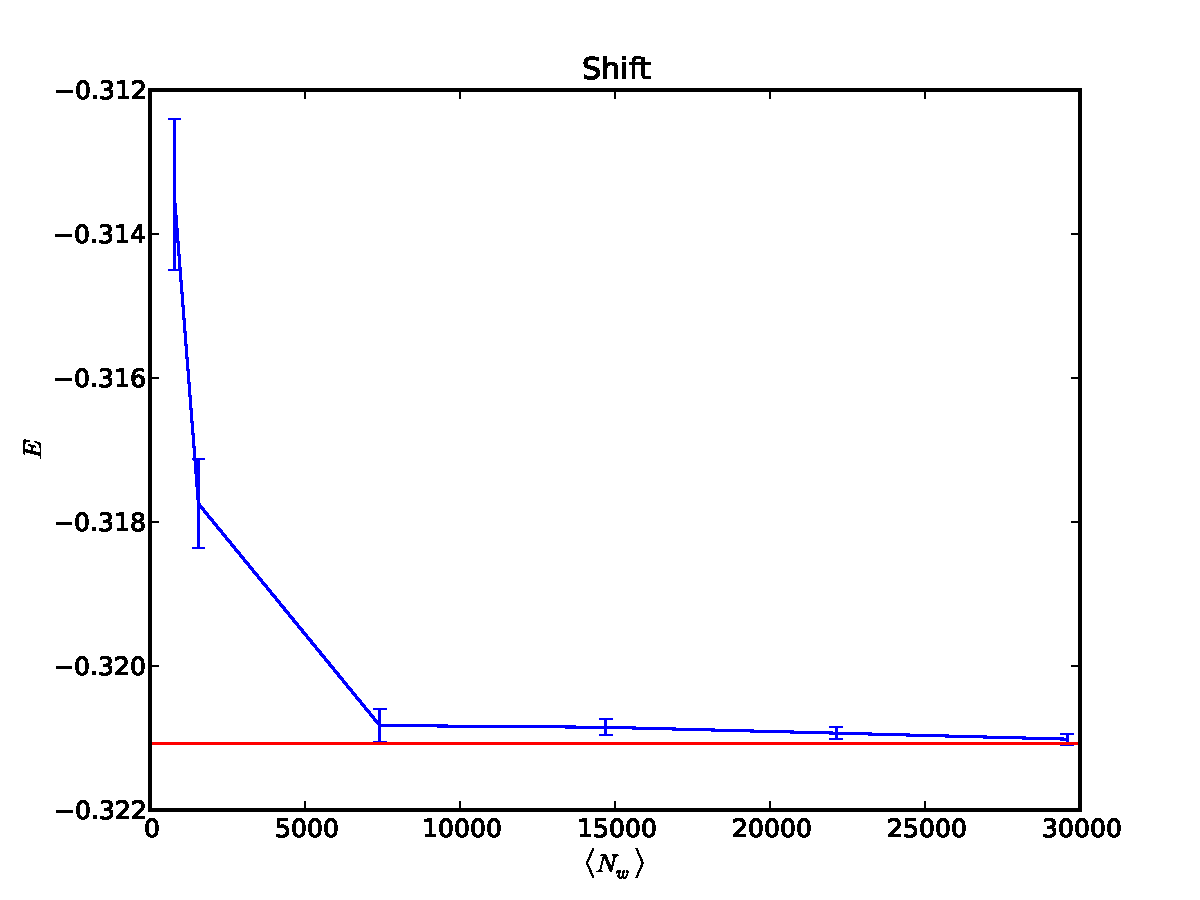
\includegraphics[width=0.5\textwidth,clip]{shift.pdf}  & 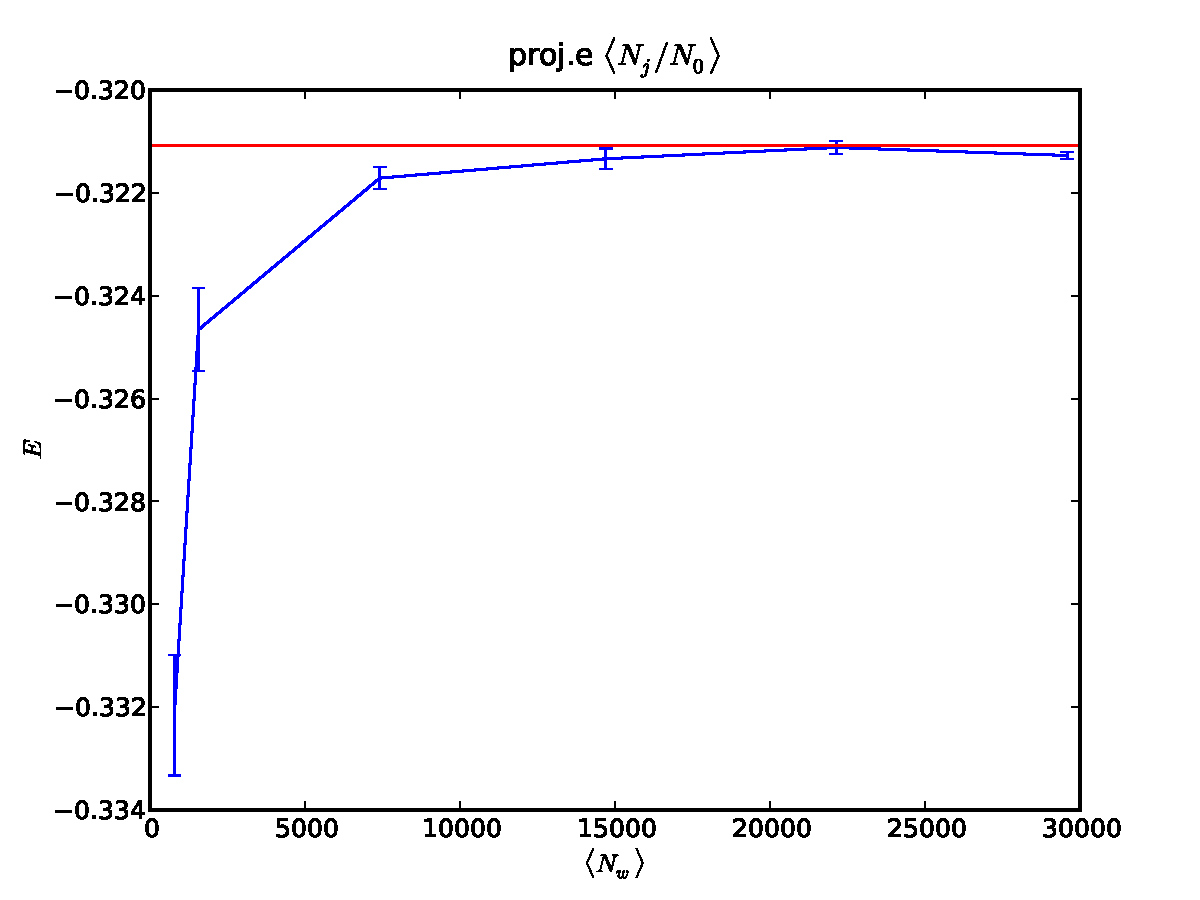
\includegraphics[width=0.5\textwidth,clip]{proje1.pdf} \\
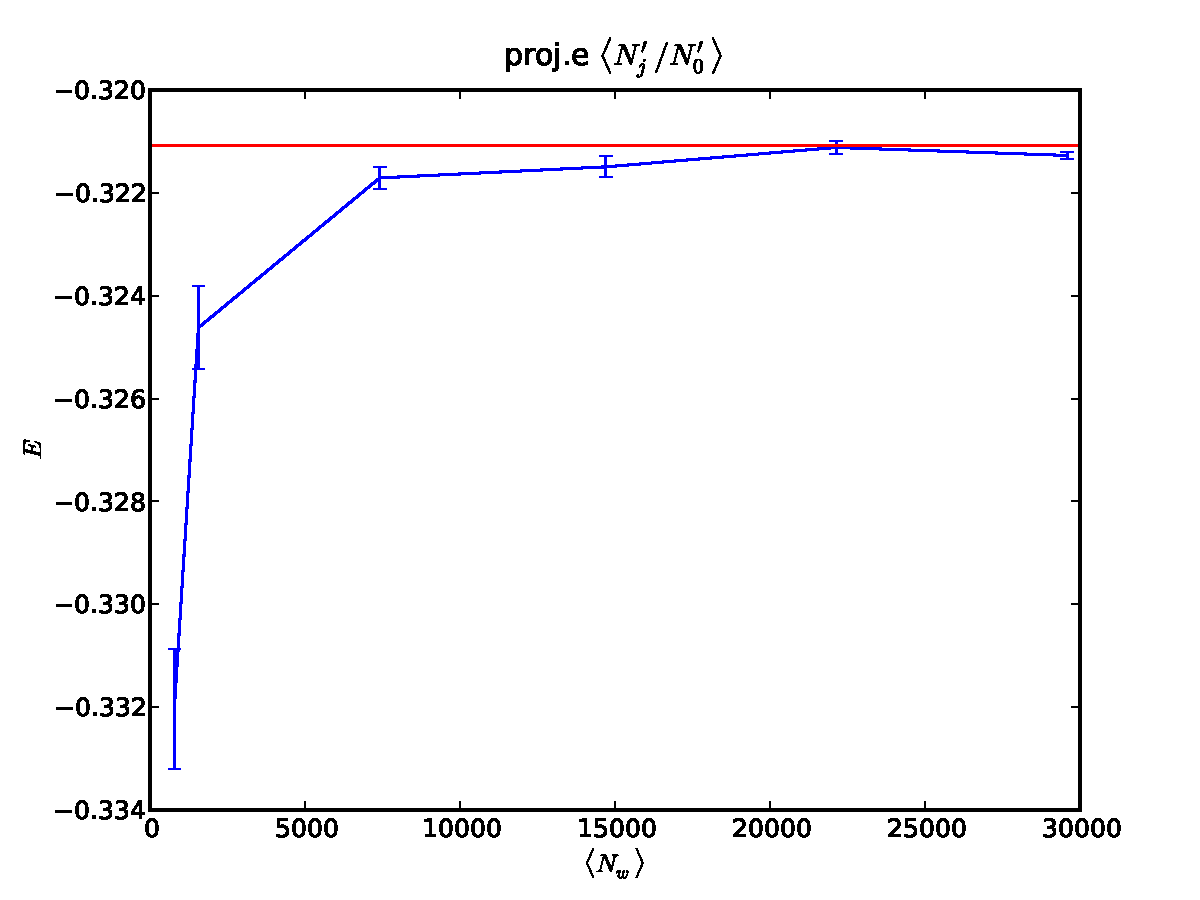
\includegraphics[width=0.5\textwidth,clip]{proje2.pdf} & 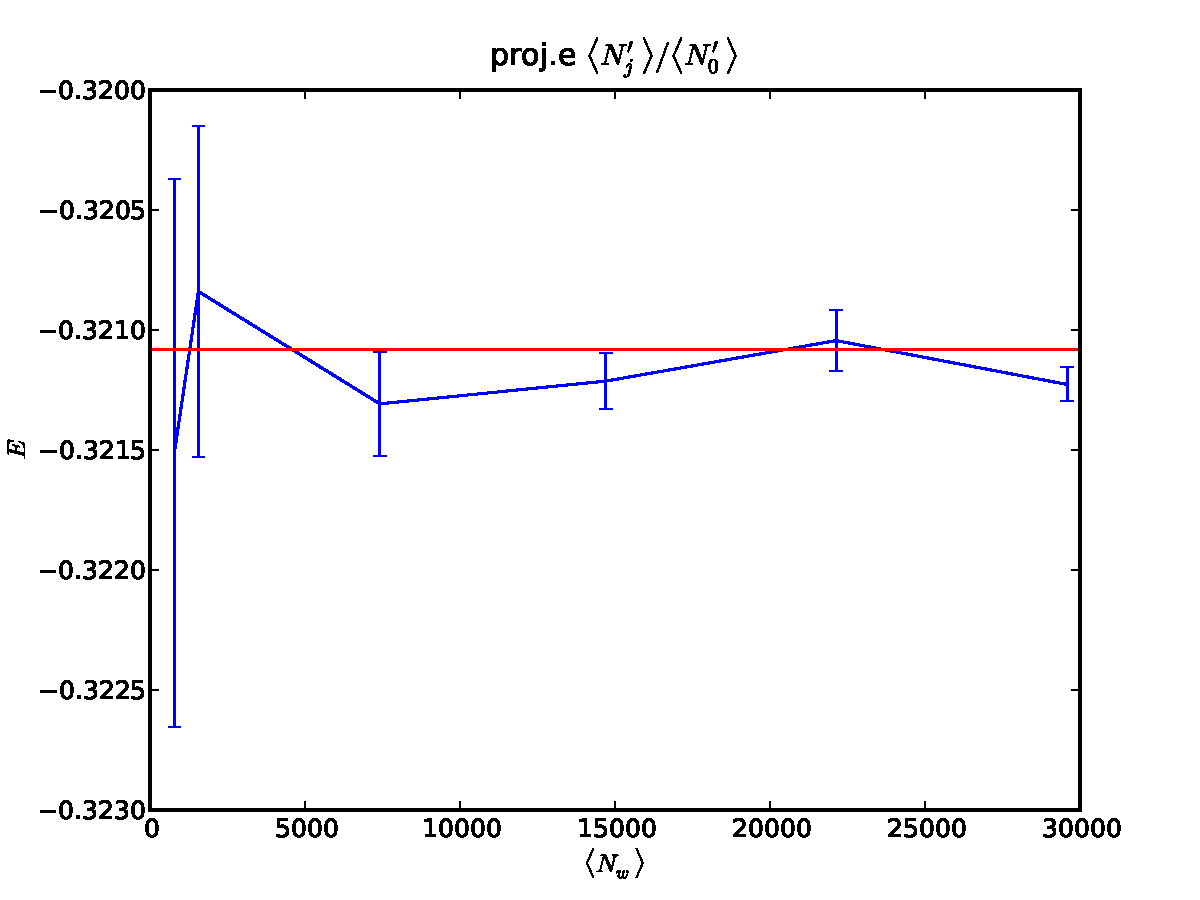
\includegraphics[width=0.5\textwidth,clip]{proje3.pdf} \\
\end{tabular}
\end{figure}

\end{document}
